\documentclass{article}
\usepackage[usenames,dvipsnames]{xcolor}
\usepackage{geometry}
\usepackage[document]{ragged2e}
\usepackage{csquotes}
\usepackage{hyperref}
\usepackage{graphicx}
\usepackage{todonotes}
\usepackage{enumitem}



\newcommand{\comment}[2]{
	\todo[color=GreenYellow,inline]{
		\underline{\textbf{#1:}} #2
	}}
% \geometry{a4paper,total={170mm,257mm},left=20mm,top=20mm}
\newcommand\independent{\protect\mathpalette{\protect\independenT}{\perp}}
\def\independenT#1#2{\mathrel{\rlap{$#1#2$}\mkern2mu{#1#2}}}

\title{Bayesian Network Exploratory Tool}
    % \today
    \author{Elad Cohen}
\begin{document}
\maketitle
    %\begin{titlepage}
    %    \begin{center}
    %       \vspace*{1cm}
    %        
    %        \textbf{Probabilistic Models Project Proposal}
    %        
    %        \vspace{0.5cm}
            
            
    %        \vspace{1.5cm}
            
    %        \vfill
            
    %        Final Project\\
            
    %        \vspace{0.8cm}
            
            
            
    %        Computer Science\\
    %        IDC\\
    %        \today
            
    %    \end{center}
    %\end{titlepage}
    \section{Introduction}\label{sec:intro}
    %\comment{Ilan}{Tightened 1st para. Notice that every sentence now contains a clear and short statement. Also moved focus to Bayesian Networks, rather than general PGMs, since most of what you propose has to do with directed graphs.}
 %   Probabilistic Graphical Models (PGM) use a graph representation to describe complex distribution over high dimensional space. Where Every node in the graph correspond a random variable, and edges in the graph correspond to direct probabilistic interactions between variables. This representation is a set of in-dependencies holds in the distribution.\\
 %   In high dimensional distribution the graph representation encode the probability in small factors rather then over every possible assignment of the variables, and the joined distribution defined as the a product of all these factors. In this kind of representation we can define Bayesian network and Markov network distributions in a visual way. Where the Bayesian network is represented as a directed graph and Markov as undirected graph.\\
 %   This representation allow humans to better evaluate properties and semantics of a variables distribution, it can help understand unexplained or undesirable answers. In addition using the graph to analyses data, it is possible to run efficient algorithm to posterior probability of variables given the evidence of others. Another characteristic is learning from data model provides a good approximation of past experience.\\~\\
 
    Probabilistic Graphical Models (PGM) are useful constructs for describing complex probability distributions over high dimensional space.
    Bayesian networks are a common type of PGMs described using a directed graph, in which nodes correspond to random variables and edges correspond to direct dependencies between variables.
    % This representation is a set of in-dependencies holds in the distribution.\\
    The power of PGMs comes from the fact that they factor a large complex joint probability distribution into a product of much smaller probability tables.
    The graph structure allows for an intuitive visual representation of the network of dependencies between variables.
    Additionally, formulation of a high-dimensional probability distribution using PGMs enables efficient algorithms for inference from data, and even learning the underlying probability.
 
%\comment{Ilan}{slightly refined para + tightened unit description}
The main objective of this project is to develop a user-friendly software tool for constructing Bayesian networks that allows interactive exploration of different aspects and inference algorithms. This tool will be designed both for educational use in academic courses and for self exploration by scientists and developers in the industry. The proposed software tool will contain six main functional units (see Section \ref{sec:design} for more detailed description):
    \begin{enumerate}
        \item Unit 1 - conditional independence in Bayesian networks (D separation criterion).
        \item Unit 2 - undirected representations of Bayesian networks and the concept of triangular (or chordal) graphs.
        \item Unit 3 - elimination orders. Examine the influence of elimination order on the complexity of the underlying inference algorithm.
        \item Unit 4 - inference algorithms. Inferring conditional distributions given observed data using elimination and message passing.
        \item Unit 5 - parameter inference.
        \item Unit 6 - sampling algorithms on Bayesian networks (MCMC, loopy belief propagation).
    \end{enumerate}
    % These units are described in greater detail in Section \ref{sec:design} below. The tool designed to experiment basic understanding from dependencies of random variables, until % running different algorithms on Bayesian networks.\\~\\

%\comment{Ilan}{need to organize this a bit more. You should describe the most relevant tools (I think ``Bayesian DAG learning'' and ``Probabilistic Graphical Models''), and list the features they support. Then in-line in the text you can mention other relevant tools. Also, use citations to connect a tool to its formal source, e.g., \cite{KevinMurphy}}
    
    There are several existing software tools for PGMs:
    \begin{enumerate}
        \item Bayesian DAG learning \cite{KevinMurphy} - Bayesian inference about directed acyclic graph (DAG) structures using dynamic programming and MCMC (Markov Chain Monte Carlo). This tool is free and it's written in Matlab. The main objective is to facilitate computation, designed to run on small amount of variables (up to 20). It's main features are:
        \begin{enumerate}
            \item Computes exact edge marginals using Bayesian model averaging with dynamic programming
            \item Computes edge marginals approximately using MCMC
        \end{enumerate}
        \item Probabilistic Graphical Models \cite{Probabilistic Graphical Model Library} - Inference of Bayesian networks and Markov chains. This tool includes learning examples as well. Implemented in Matlab with following features:
        \begin{enumerate}
            \item Joint distribution calculation
            \item Marginal distribution calculation
            \item Maximum probability assignment calculation
            \item Inference on tree structured network
        \end{enumerate}
        %\item Kevin Murphy - THe most comprehensive tool we found, an assemble of Matlab libraries implements various probabilistic models. Most of the libraries written by Kevin Murphy along with his students. Some of the libraries are:
        %    \begin{enumerate}
        %        \item PMTK - A collection of Matlab functions, written to support Kevin Murphy textbook ``Machine learning: a probabilistic perspective''.
        %        \item DAG structure learning using L1 regularization - A library to find Markov blankets using L1
        %        \item Bayesian DAG learning - Bayesian inference over DAG (directed acyclic graph). This library cannot handle undirected graphs and inference with hidden nodes.
        %    \end{enumerate}
        %\item Hidden Markov Model Toolbox - Written By Kevin Murphy in 1998, support inference for HMMs (Hidden Markov Model), implemented on Matlab
        %\item OpenGM - A C++ Implementation for discrete factor graph models. The main objective of this library is to give efficient implementation, and not a learning experience.
        %\item Probabilistic Graphical Models - A Matlab implementation for inference and learning Bayesian and Markov networks hosted on Github. The library gives a code to learn PGM, but lack the visualization part.
    \end{enumerate}

    Other relevant tools, e.g OpenGM \cite{OpenGM} (Discrete factor graph models), Hidden Markov Model Toolbox \cite{Hidden Markov Model Toolbox} ( Hidden Markov Model), MAP estimation of DAG structure \cite{MAPEstimation}, are more specialized and do not contain the main features of our proposed tool.
 
    In summary, existing libraries have some aspects in common with our tool, but none of them appear to have the interactive nature that will support friendly exploration and learning. Additionally, none of these tools possess the gradual unit structure we propose, which we believe will help convey complex concepts in statistical learning.
    
    
    \section{Proposed Design}\label{sec:design}
    %\comment{Ilan}{Shortened here. Note that every sentence contains a succinct and clear statement. Minor statements can be removed.}
    The software tool will consist of six sequential functional units. A Bayesian network is represented via a directed acyclic graph, where each node represents a random variable, with conditional distribution table given its parents (or predecessors) in the graph. The visual representation of the graph allows users to explore the network and observe the different conditional distribution tables.
    
    % Before we dive into every unit, let us define the basic capability this tool, give the user the ability to define a Bayesian network in two basic steps:
    % \begin{enumerate}
    %     \item Define all nodes of the network that represent random variables
    %     \item For every node the user is able to define it's parents. Where a node can have 0 or more parents
    % \end{enumerate}
    % This way the user is able to visual his network as a directed graph and explore it.
    \begin{enumerate}
        \item Unit 1\label{unit1} -- 
        % This unit is the designed to learn the basics of probabilistic models through a visual representation of Bayesian network, as a directed graph without the probability definition of every node.
       fundamental concept of conditional independence in Bayesian networks. This unit considers only the graph structure of the network and ignores the probability tables.
       %\comment{Ilan}{added marginal independence here. It's a special case, but you can mention it as a separate feature.}
        \begin{enumerate}
            \item Marginal independence. The user selects two nodes in the network, and the program specifies whether they are independent or not. If they are dependent, then the connecting path is highlighted.
            \item Conditional independence. The user selects two nodes $u,v$ and a set of nodes to condition on $A$, and the program specifies whether $X_u$ and $X_v$ are conditionally independent given the collection $X_A$ ($X_V \independent X_U | X_A$). We will use the D-separation criterion for this and highlight the path that blocks dependence.
            
            %, using D separation criteriation. The D separation is a general criterion for deciding from a given graph whether a set of variables X are independent of another set U %given another set A. Or more formally: $X_V \independent X_U | X_A$.\\
            %The user is going to be able to choose two nodes to check independence for, and a set of nodes to condition on, all on the graph representation of Bayesian network. The tool is going to show if those nodes are independent. Highlight on the graph the paths that block dependency
        \end{enumerate}

        \vspace{0.5cm}
%\comment{Ilan}{tweaked here. This was quite good!}
        \item Unit 2\label{unit2} -- 
%        This unit objective is understanding the undirected graph representation of the Bayesian network. In the unit we are still not taking the probability of the nodes into 
%	 consideration for all operations. 
        undirected graph representation of Bayesian networks.  This unit also considers only the graph structure of the network and ignores the probability tables.
        \begin{enumerate}
            \item 
             %In one click the user can
             Convert the directed graph representation to an undirected graph, called the moralized graph. In this undirected representation parents of a node in the original graph will have a new edge between them. %This emphasize the fact that
             Consequently, all variables in the same conditional probability table form a clique.
            \item %Validate if
            Examine whether the moralized graph is chordal (triangulated) or not. %The main characteristic of this graph is that
            In a chordal graph, every cycle of four or more vertices %have
            has a chord. %, in other words every included cycle in the graph should have exactly three vertices. 
            %This representation can help the user understand if 
            Note that a perfect elimination exists, iff the moralized graph is chordal (see Unit 3).
            \item Convert the moralized graph into a factor graph -- a bipartite graph representation with one class representing nodes in original graph and the other class representing maximal cliques (probability distribution tables).
        \end{enumerate}
        
        
%\comment{Ilan}{I stopped direct edits at this point. Please implement edits based on style of previous units.}
 
 %\comment{Ilan}{we keep returning to this issue - unit 3 is about elimination orders. Not inference yet, and no use of actual probability tables. Please fix. I also think that you should specify two modes: one where the user iteratively selects nodes for elimination, and the other, where the program searches for a perfect order, until it gets stuck, and the user has to select the next node, etc.}
        \item Unit 3\label{unit3} -- 
            Elimination algorithm on undirected graph. Helps choose an elimination order for the purpose of inference without carrying out the complex computations of the probability tables.
        \begin{enumerate}
            \item Show elimination algorithm implementation on graphs. User can run elimination algorithm step by step. On every step the user choose a node to eliminate, on the graph the user can see the new edges added to the graph.
            \item Try to find a prefect elimination order, choose one simplical node and start elimination from there, write the order on the screen, on every step find the next simplical node, if there is not such one, the user will be able to choose the next node to eliminate.
        \end{enumerate}
 %\comment{Ilan}{you can definitely add more details here. The user has to select the observed variables and the observed values. Then the program computes marginal probabilities or max-prob assignments. Also mention different modes of inference - simple elimination, message passing, parallel message passing. This is actually the unit that should be fleshed out the most, because it is the core of the program.}
        \item Unit 4 --
            Inference of hidden variables using observed variables. In this unit the main objective is to show calculation of joint, marginal and max probability of random variables. Show inference on graph representation (undirected, factor) of Bayesian network along with probability tables. Inference starts by the user selecting as first step the user selects the observed nodes on the network, for each one sets the node value (for elimination algorithm choose the nodes to inference).

            Inference then proceeds using one of three possible procedures:
            \begin{enumerate}
                \item Simple elimination - find marginal distribution for a set of variables given another set of observed variables.
                \item Message Passing - compute marginal distribution for several variables separately given a set of observed variables.
                \item Parallel Message Passing - same computation as in the last item but run the procedure in parallel (cannot run the step by step execution mode)
            \end{enumerate}

            The message passing algorithm (sequential or parallel) can be used to make one of two possible calculations:
            \begin{enumerate}
                \item Marginal distribution - calculates marginal distribution for every node
                \item Max probability assignment - computes assignment of unobserved nodes with observed nodes 
            \end{enumerate}

            All inference procedures can be run automatically (user just see the end result), or step-by-step to allow users to follow the calculations.

            %\comment{Elad}{Another thing i wanted to add (let me know if you think we need to add it): The user can choose to see algorithms run on undirected graph or factor graph representation of the Bayesian networks}
        \item Unit 5 --
            Parameter inference from data. The networks this unit is operating on are HMM (Hidden Markov Model) and small Bayesian network with many independent copies.

            The user has the ability to choose a couple of modes:
            \begin{enumerate}
                \item Inference where all nodes are observed. is data to sufficient statistics table and display it to the user.
                \item Inference where some of the nodes are observed and some are hidden using:
                \begin{enumerate}
                    \item Maximum probability inference
                    \item EM (expectation maximization) 
                \end{enumerate}
            \end{enumerate}
        \item Unit 6 --
            Other advanced algoriths such as:
        \begin{enumerate}
            \item Markov chain Monte Carlo algorithm
            \item Loopy Belief Propagation 
        \end{enumerate}
    \end{enumerate}

    \section{Implementation Demo}\label{sec:demo}
    For a demonstration of the tool, we constructed a Bayesian network with 5 binary random variables, and added dependencies between them (see figure \ref{fig:besian_network}). Figure \ref{fig:besian_network} illustrates that conditional distribution table of variable ($X_4$) is displayed when its vertex in the network is selected via mouse click.\\

    The Binary membership table have two dimensions, one shows all the probability functions one random variable participant in, the second shows all random variables of one probability function. Figure \ref{fig:binary_membership} shows the binary membership table for this network.
    Another important feature of the tool is the ability to examine the undirected version of the graph, moralized graph (Figure \ref{fig:moralized_graph}; unit \ref{unit2}).
    Note that in our network the moralized graph is not chordal, there is a simple cycle of 4 without a chord ($X_1, X_2, X_3, X_4$).
    Next we can start an elimination process by selecting one vertex in the graph ($X_4$), we can see how it is eliminated from the graph and new edges introduced in the undirected graph representation of the network (figure \ref{fig:elimination}; unit \ref{unit3}). Binary membership table also changed, all probability functions this variable participant in replaced by the new probability function introduced in the elimination.

    \section{Work plan}
    Next step is implementation of the tool, right now there is a proof of concept of the tool and all screen shots on this proposal taken from there. Implementation of the to will be sequential by the units (unit 1, unit 2 ...), since every unit adds new capabilities to former one. But before all units, we are going to implement the UI to define a Bayesian network.\\ Theoretical and user guide documentation for every unit are written along with the unit implementation.

    This tool have two part, UI and server (support heavy operations on the network). As part of the tool we will use different open source libraries. 
    \begin{enumerate}
        \item UI - Using browser for display, so languages are Javascript, CSS, HTML. The open source project we are using to support our tool are: React, Redux, Vis.js (Graph library), DataTables (HTML table library).
        \item Server - Written in Java. Using Spring boot as framework for DI (dependency injection) and to create executable JAR.
    \end{enumerate}

    This tool will have two predefined networks, the user can use them instead of defining a new network. The structure of the networks are:
    \begin{enumerate}
        \item Small Bayesian network with 6 random variables. This network is not chordal in it's moralized representation.
        \begin{figure}[hb!]
            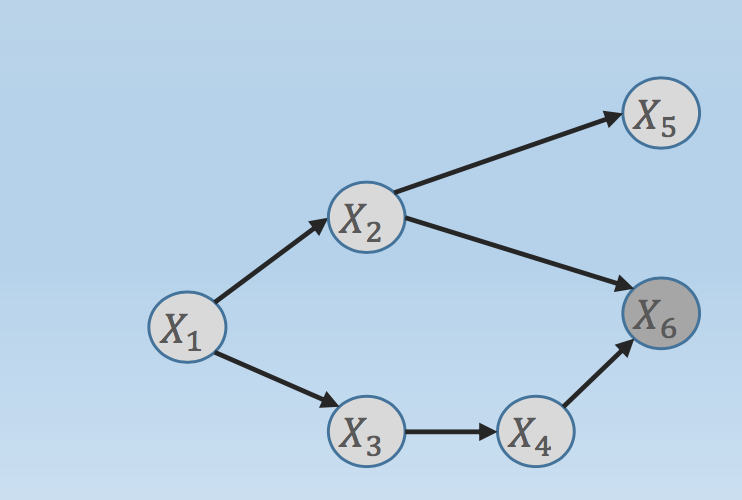
\includegraphics[width=\textwidth]{img/small_network.png}
            \centering
            \caption{Six random variable Bayesian network representation using directed graph}
            \label{fig:simple_network}
        \end{figure}
        \item Network with length parameter N, with three variables X, Y, Z, where X and Y dependent on N. Dependencies in the network: $\forall y_i \in Y, i>0 P(y_i | y_{i-1})$, $\forall x_i \in X P(x_i | Y_i, Z)$ figure \ref{fig:parameterized_network}. In figure \ref{fig:parameterize_network_description} we can see the conditional table.
        \begin{figure}[hb!]
            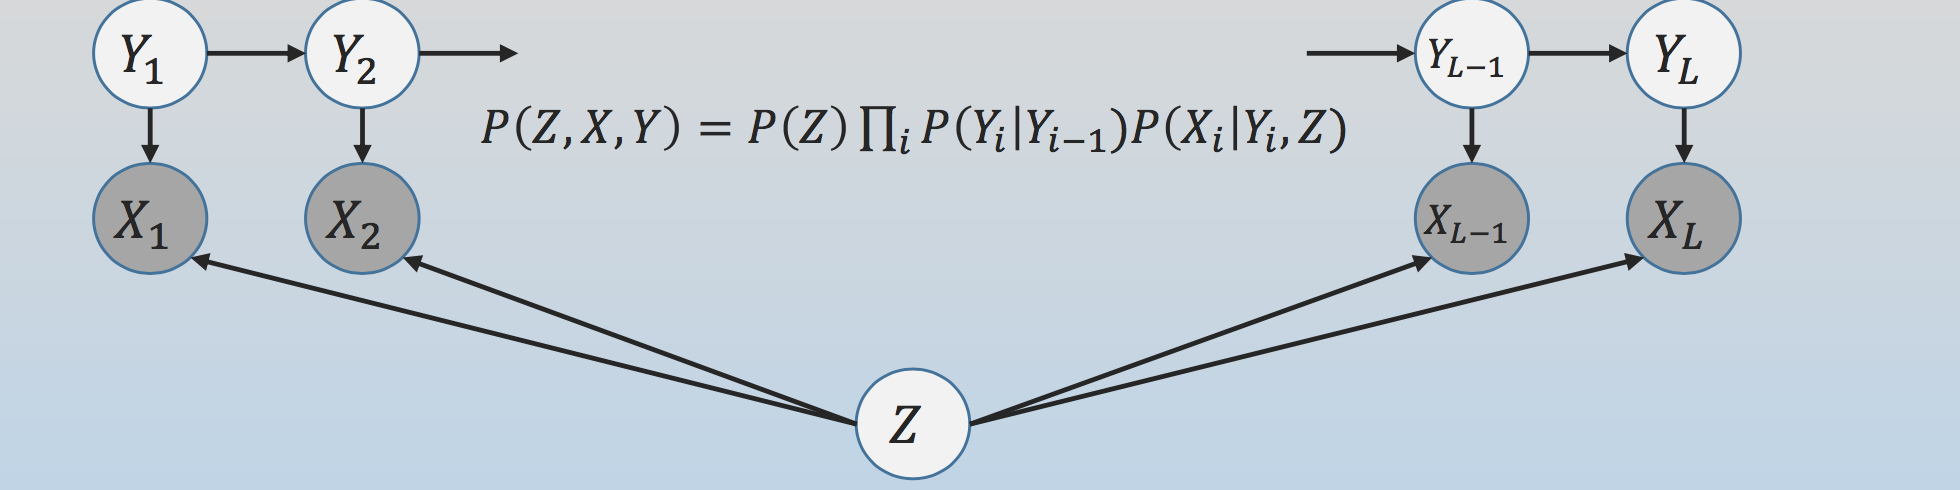
\includegraphics[width=\textwidth]{img/iterative_network.png}
            \centering
            \caption{Parameterize network}
            \label{fig:parameterized_network}
        \end{figure}
        \begin{figure}[hb!]
            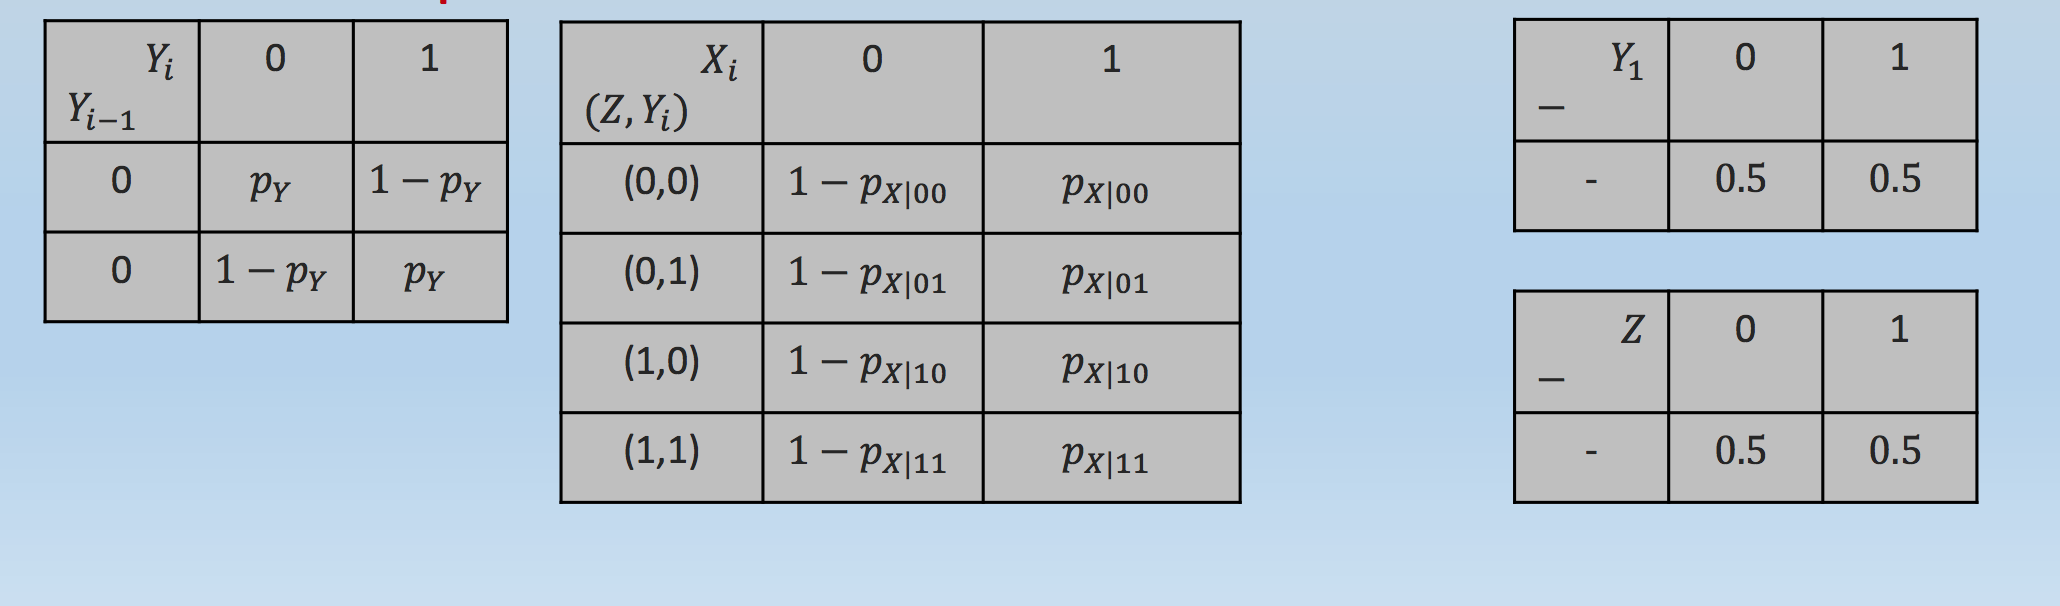
\includegraphics[width=\textwidth]{img/parameterize_network_description.png}
            \centering
            \caption{Parameterize network probability tables}
            \label{fig:parameterize_network_description}
        \end{figure}
    \end{enumerate}

    \begin{figure}[hb!]
        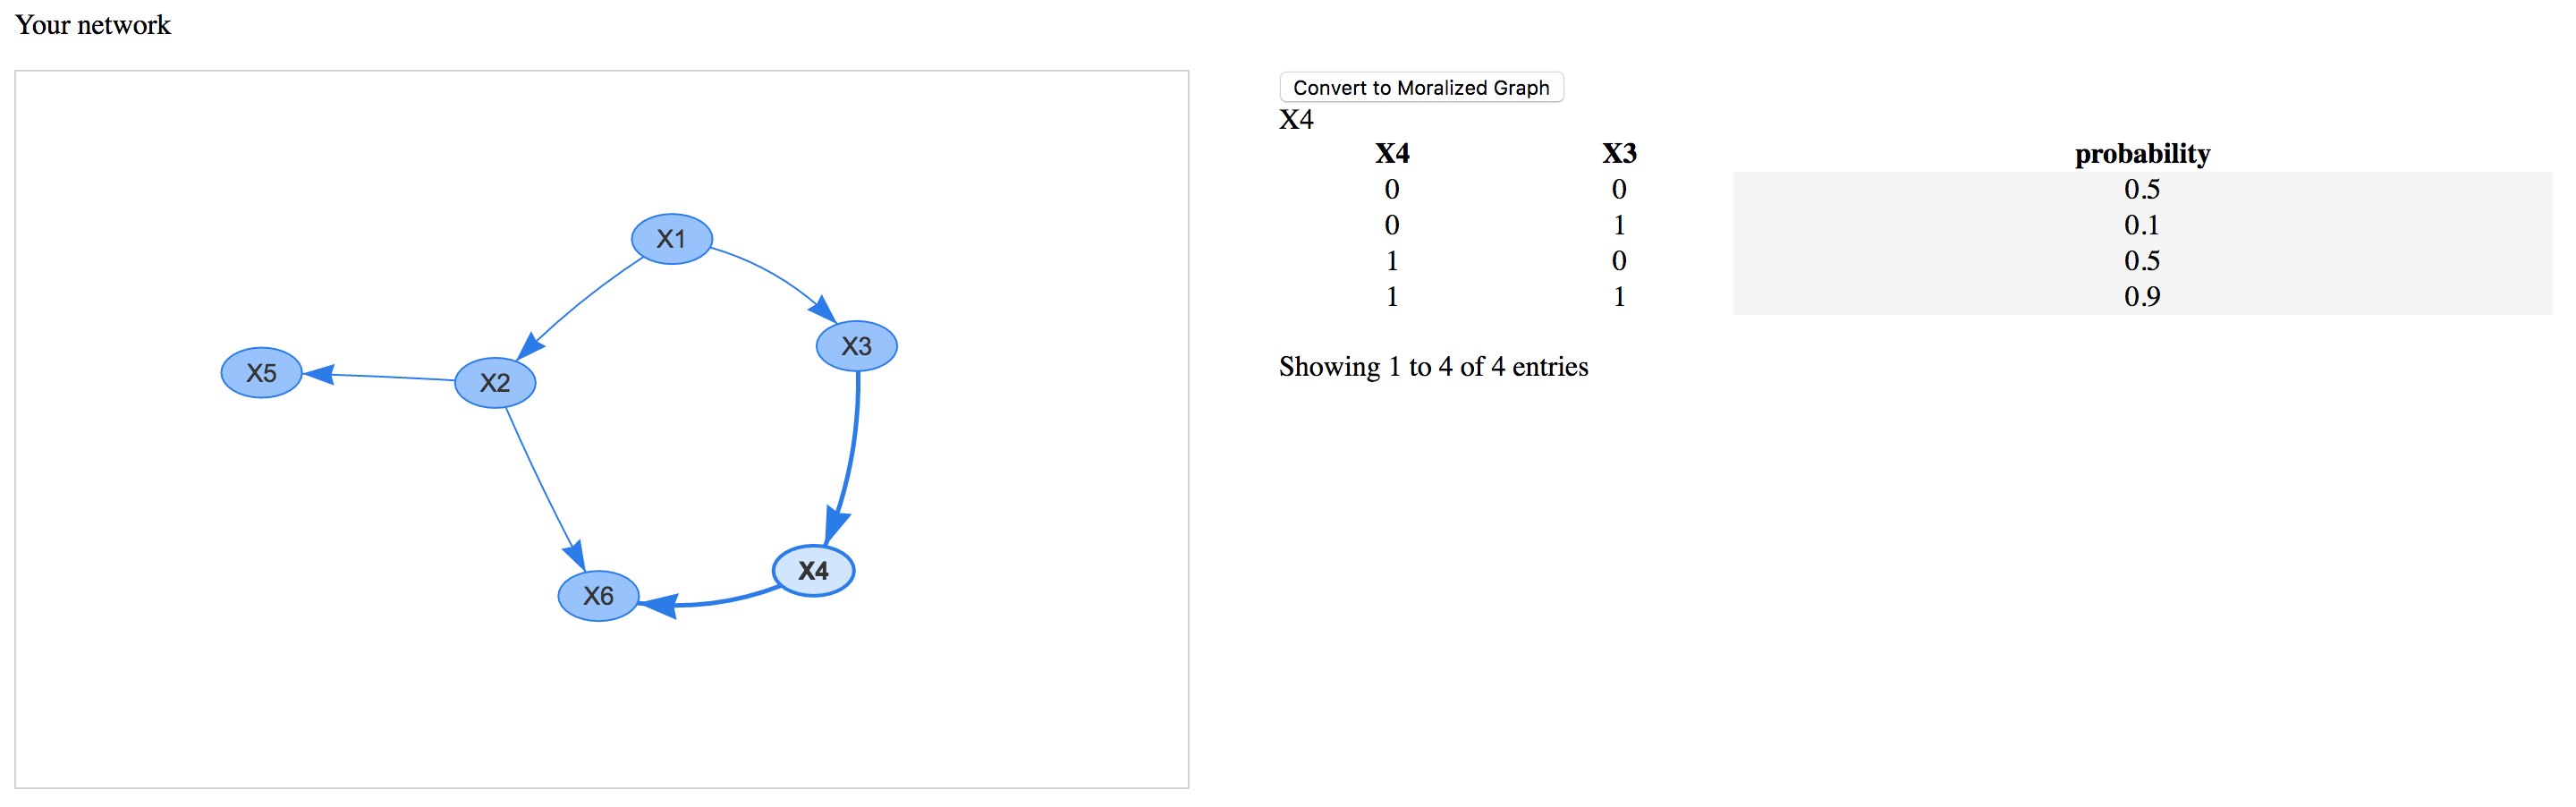
\includegraphics[width=\textwidth]{img/network_one_highlighted.png}
        \centering
        \caption{A simple Bayesian network representation using directed graph}
        \label{fig:besian_network}
    \end{figure}

    \begin{figure}[hb!]
        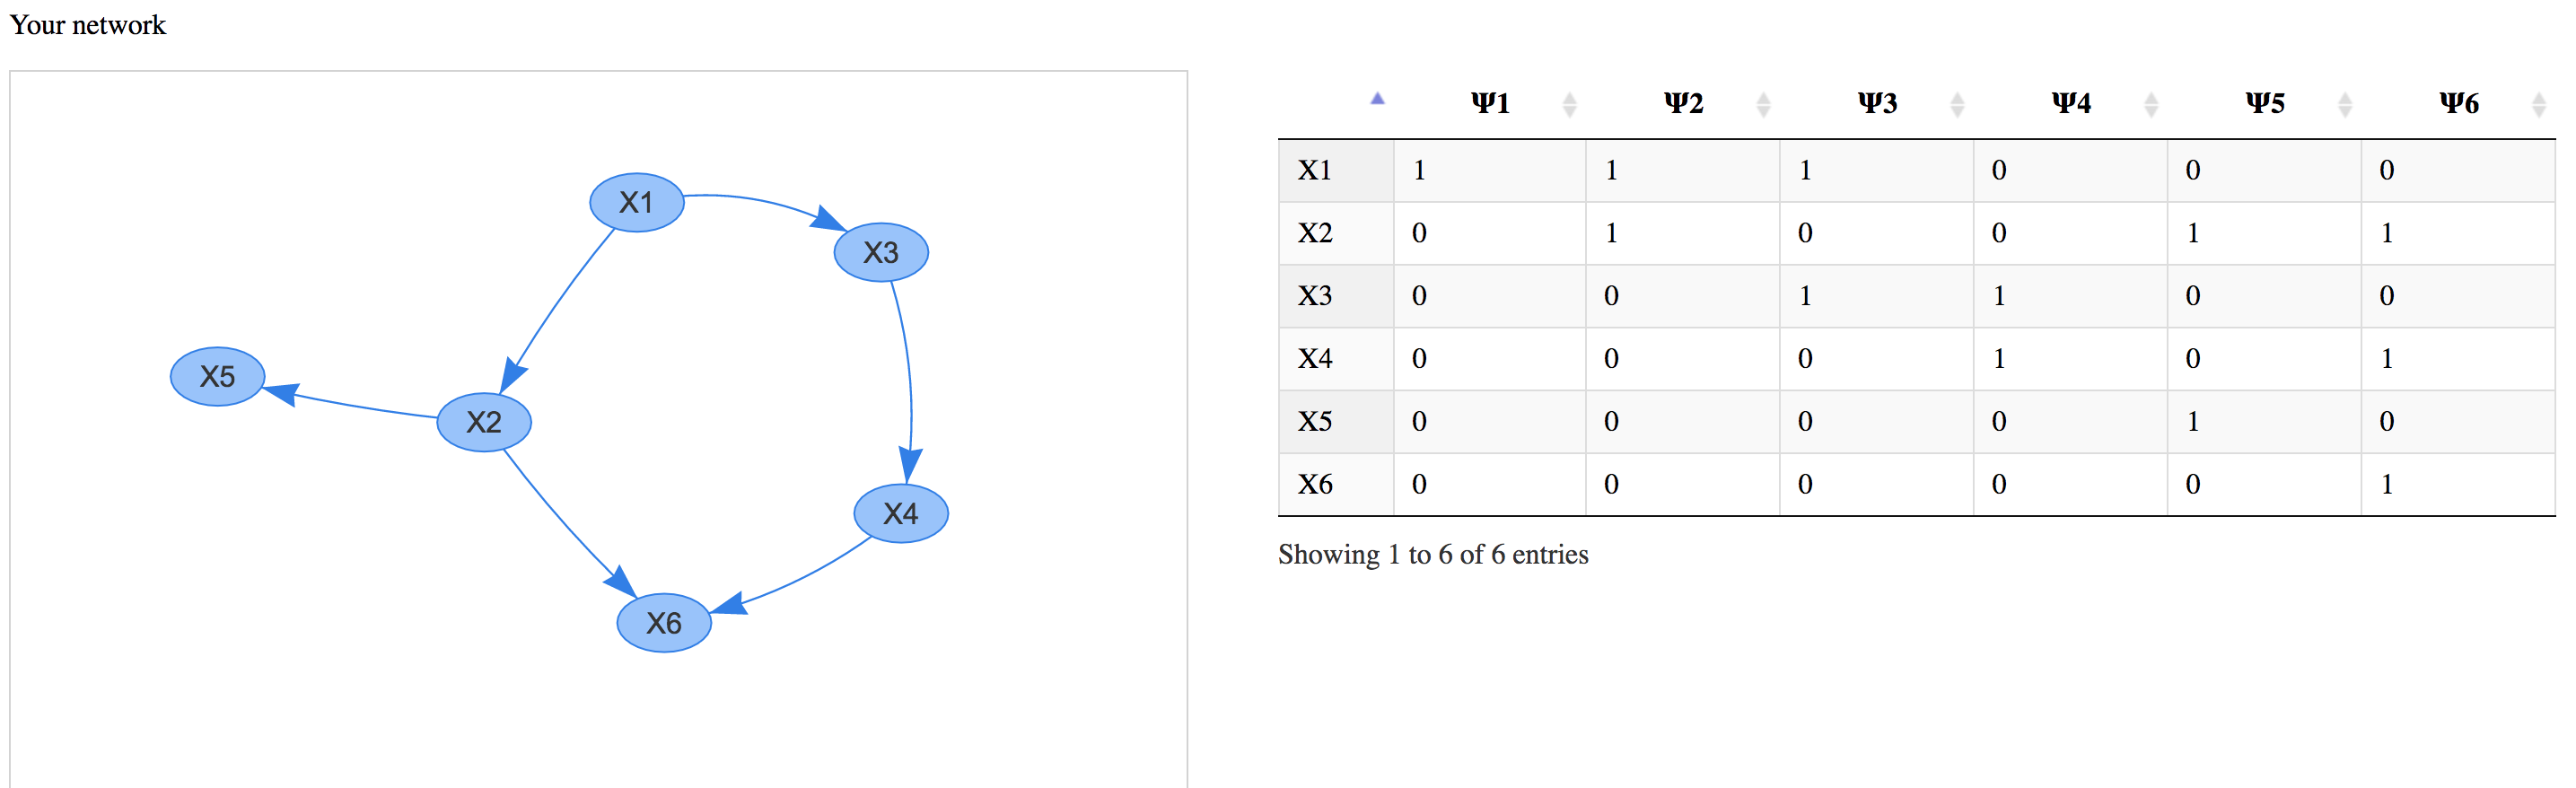
\includegraphics[width=\linewidth]{img/network_binary_matrix.png}
        \caption{Showing binary membership table of the network}
        \label{fig:binary_membership}
    \end{figure}

    \begin{figure}[hb!]
        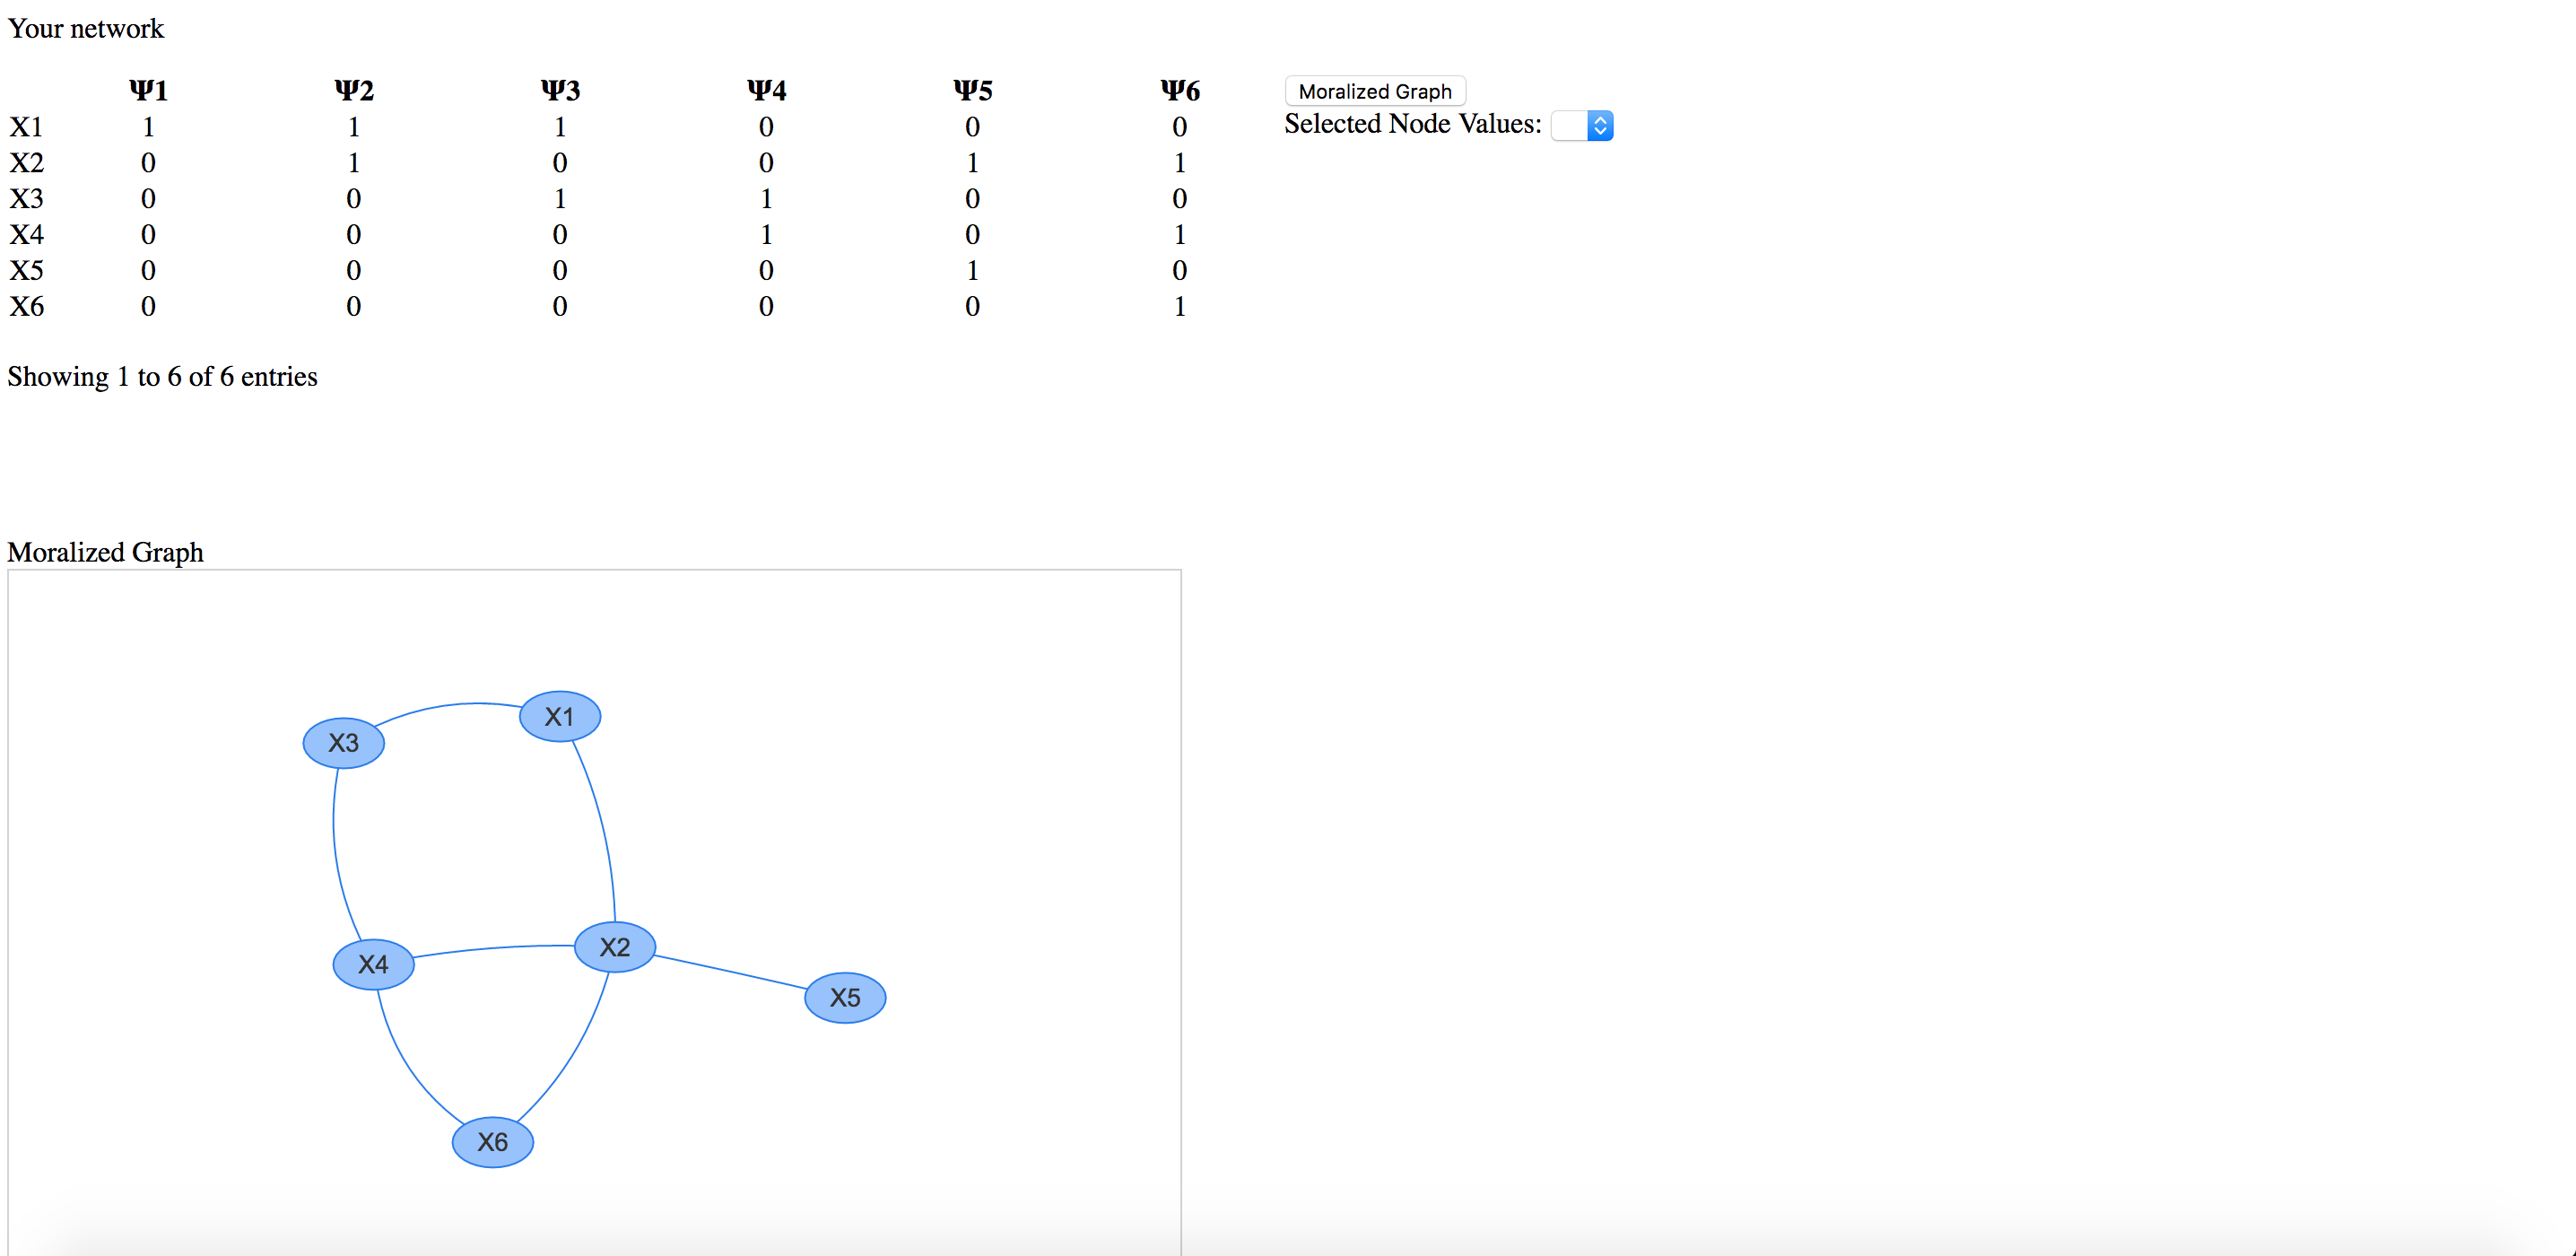
\includegraphics[width=\linewidth]{img/moralized_graph.png}
        \caption{Moralized Graph representation}
        \label{fig:moralized_graph}
    \end{figure}

    \begin{figure}[hb!]
        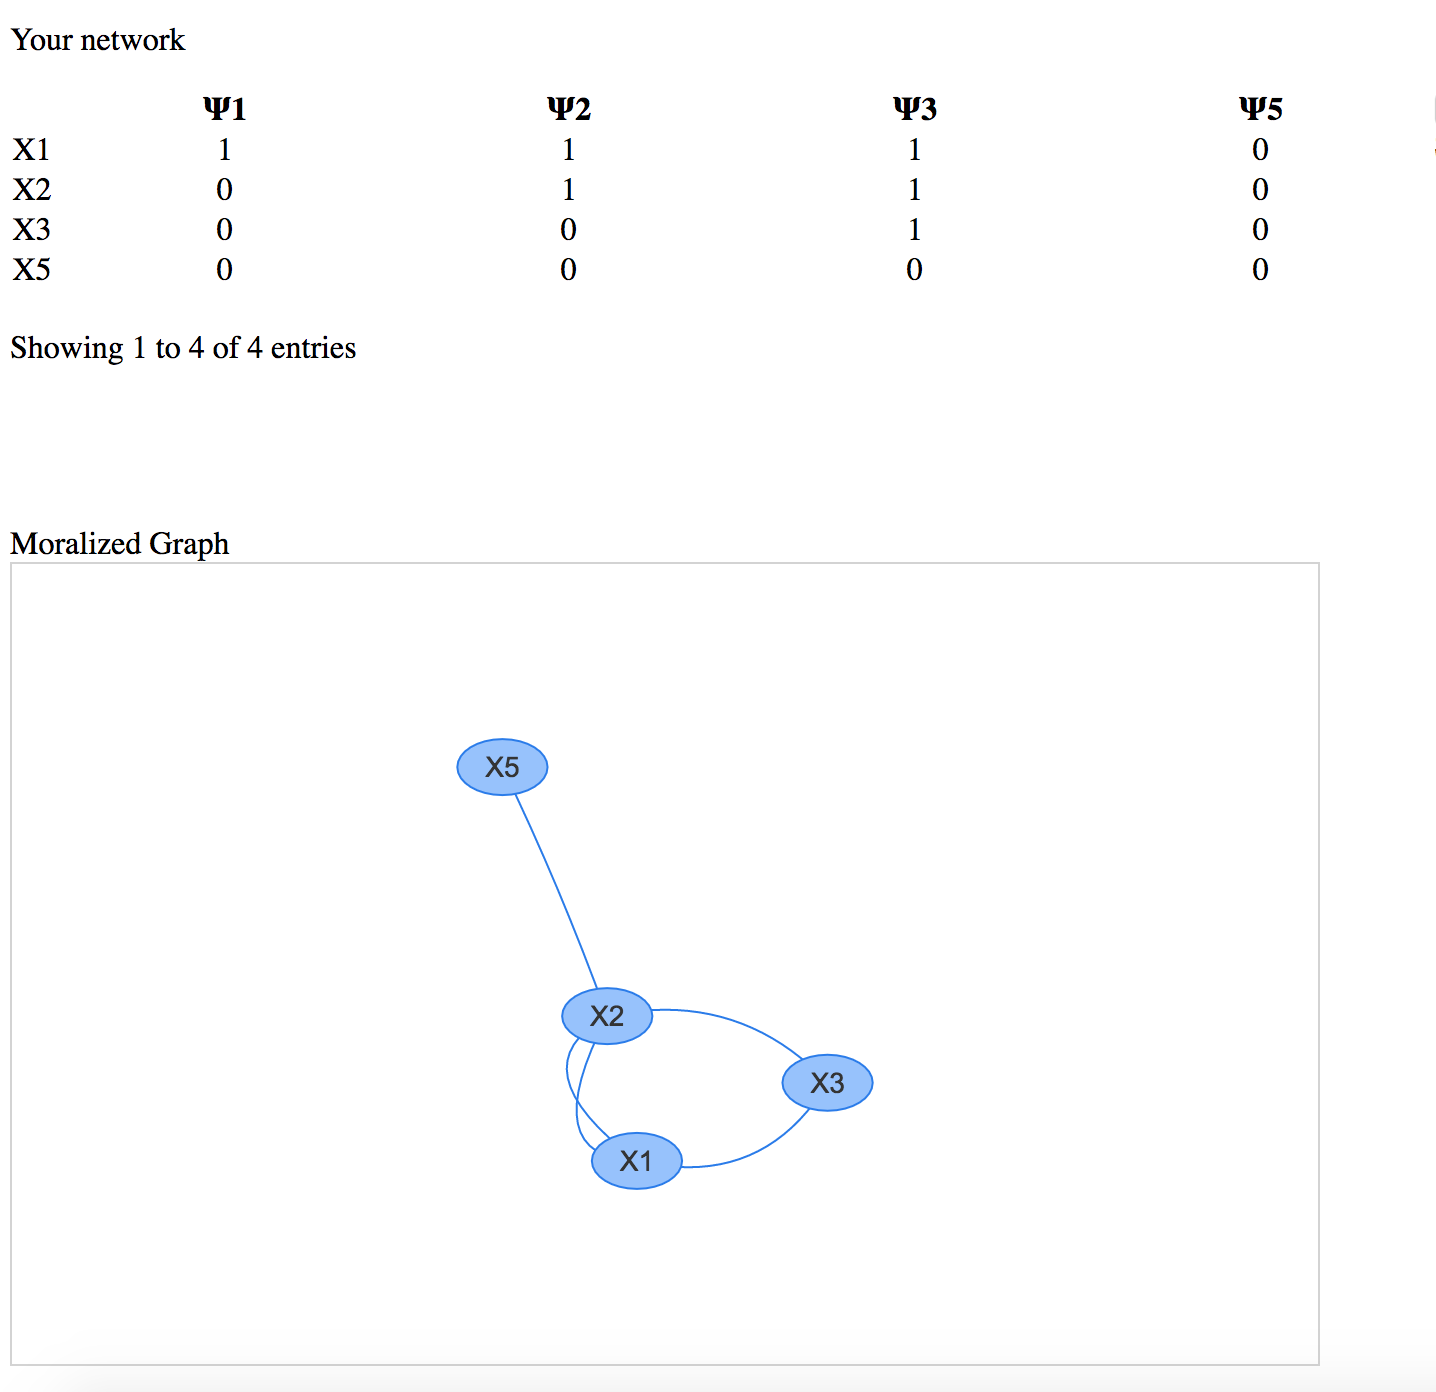
\includegraphics[width=\linewidth]{img/after_x4_elimination.png}
        \caption{After X4 is eliminated from the graph. We can see a new edge was created between X2 and X3. Now X5 node is chosen to be eliminated next}
        \label{fig:elimination}
    \end{figure}

    % \newpage
    \begin{thebibliography}{5}
        \bibitem{KevinMurphy}
        Kevin Murphy, PGM Matlab libraries, \\\texttt{http://www.cs.ubc.ca/\~{}murphyk/Software/}
        \bibitem{Hidden Markov Model Toolbox}
        Kevin Murphy, toolbox for inference on Hidden Markov Models, \\\texttt{http://www.cs.ubc.ca/\~{}murphyk/Software/HMM/hmm.html}
        \bibitem{OpenGM}
        Bjoern Andre, Thorsten Beier and Joerg H. Kappes, OpenGM, \\\texttt{http://hciweb2.iwr.uni-heidelberg.de/opengm/}
        \bibitem{Probabilistic Graphical Model Library} 
        Syllogismos, PGM learning, \\\texttt{https://github.com/anhncs/Probabilistic-Graphical-Models}
        \bibitem{MAPEstimation}
        Mark Schmidt and Kevin Murphy, MAP estimation  of DAG structures, \\\texttt{http://www.cs.ubc.ca/~murphyk/Software/DAGlearn/index.html}
    \end{thebibliography}
\end{document}